\documentclass[a4paper,11pt]{article}
\usepackage{amsmath,amsthm,amsfonts,amssymb,amscd,amstext,vmargin,graphics,graphicx,tabularx,multicol} 
\usepackage[francais]{babel}
\usepackage[utf8]{inputenc}  
\usepackage[T1]{fontenc} 
\usepackage{pstricks-add,tikz,tkz-tab,variations}
\usepackage[autolanguage,np]{numprint} 
\usepackage{calc}
\usepackage{amssymb}
\usepackage{enumitem} 

\setmarginsrb{1.5cm}{0.5cm}{1cm}{0.5cm}{0cm}{0cm}{0cm}{0cm} %Gauche, haut, droite, haut
\newcounter{numexo}
\newcommand{\exo}[1]{\stepcounter{numexo}\noindent{\bf Exercice~\thenumexo} : }
\reversemarginpar

\newcommand{\bmul}[1]{\begin{multicols}{#1}}
\newcommand{\emul}{\end{multicols}}

\newcounter{enumtabi}
\newcounter{enumtaba}
\newcommand{\q}{\stepcounter{enumtabi} \theenumtabi.  }
\newcommand{\qa}{\stepcounter{enumtaba} (\alph{enumtaba}) }
\newcommand{\initq}{\setcounter{enumtabi}{0}}
\newcommand{\initqa}{\setcounter{enumtaba}{0}}

\newcommand{\be}{\begin{enumerate}}
\newcommand{\ee}{\end{enumerate}}
\newcommand{\bi}{\begin{itemize}}
\newcommand{\ei}{\end{itemize}}
\newcommand{\bp}{\begin{pspicture*}}
\newcommand{\ep}{\end{pspicture*}}
\newcommand{\bt}{\begin{tabular}}
\newcommand{\et}{\end{tabular}}
\renewcommand{\tabularxcolumn}[1]{>{\centering}m{#1}} %(colonne m{} centrée, au lieu de p par défault) 
\newcommand{\tnl}{\tabularnewline}

\newcommand{\trait}{\noindent \rule{\linewidth}{0.2mm}}
\newcommand{\hs}[1]{\hspace{#1}}
\newcommand{\vs}[1]{\vspace{#1}}

\newcommand{\N}{\mathbb{N}}
\newcommand{\Z}{\mathbb{Z}}
\newcommand{\R}{\mathbb{R}}
\newcommand{\C}{\mathbb{C}}
\newcommand{\Dcal}{\mathcal{D}}
\newcommand{\Ccal}{\mathcal{C}}
\newcommand{\mc}{\mathcal}

\newcommand{\vect}[1]{\overrightarrow{#1}}
\newcommand{\ds}{\displaystyle}
\newcommand{\eq}{\quad \Leftrightarrow \quad}
\newcommand{\vecti}{\vec{\imath}}
\newcommand{\vectj}{\vec{\jmath}}
\newcommand{\Oij}{(O;\vec{\imath}, \vec{\jmath})}
\newcommand{\OIJ}{(O;I,J)}


\newcommand{\reponse}[1][1]{%
\multido{}{#1}{\makebox[\linewidth]{\rule[0pt]{0pt}{20pt}\dotfill}
}}

\newcommand{\titre}[5] 
% #1: titre #2: haut gauche #3: bas gauche #4: haut droite #5: bas droite
{
\noindent #2 \hfill #4 \\
#3 \hfill #5

\vspace{-1.6cm}

\begin{center}\rule{6cm}{0.5mm}\end{center}
\vspace{0.2cm}
\begin{center}{\large{\textbf{#1}}}\end{center}
\begin{center}\rule{6cm}{0.5mm}\end{center}
}



\begin{document}
\pagestyle{empty}
\titre{Séance d'AP 5 : Le vide grenier et un peu de logique }{}{}{6ème}{}

\vspace*{0.3cm}

\exo  \\
Julien participe au vide grenier. \\ 
Il ne peut malheureusement pas amener tous les objets qu'il voudrait car son sac à dos ne peut contenir au maximum que 8 kg.  

\begin{center}
\includegraphics[scale=1]{videgrenier.eps} 
\end{center}

\textbf{Votre mission :}\\
$\rightarrow$ L'aider à remplir son sac pour qu'il puisse gagner le maximum d'argent. Vous pouvez écrire les solutions que vous trouvez et mettre en valeur celle qui est la plus intéressante.\\

\noindent \reponse[10]\\


\newpage

{\Large \textbf{C'est extra... terrestre !}}\\

\bmul{2}

\bi[label=$\blacktriangleright$]

\item Le Vénusien est bleu.

\item L'extraterrestre violet vit dans la maison sphérique.

\item Le Neptunien a deux fois plus d'orteils que le Vénusien.

\item Le Vénusien a deux fois plus d'orteils que le Martien.

\item Dans la maison cylindrique vit la tête ronde.

\item La tête carrée est violette.

\item L'extraterrestre vert ne vit pas dans la maison conique.

\item Le saturnien habite dans la maison cubique.

\item Celui qui a le plus d'orteils a une tête rectangulaire.

\item Un extraterrestre a 6, 12, 18 ou 24 orteils.

\item Aucun des extraterrestres n'a le même nombre d'orteils.

\item Celui qui a 6 orteils a la tête carrée.



\ei


\columnbreak

\includegraphics[scale=0.8]{logique.eps} 

\emul

\vspace*{1cm}

\textbf{Pour répondre aux questions suivantes, vous pouvez compléter le tableau récapitulatif juste en dessous pour vous aider.}\\

\q Qui est l'extraterrestre jaune ?\\
\reponse[3]\\

\q Qui est l'extraterrestre à la tête triangulaire ?\\
\reponse[3]\\

\vspace*{0.5cm}


\textbf{Tableau récapitulatif :}\\
\vspace*{0.3cm}


{\renewcommand{\arraystretch}{2}
\begin{flushleft}
\begin{tabular}{|c|c|c|c|c|}
\hline 
 & \hspace*{0.5cm} \textbf{Vénusien} \hspace*{0.5cm} &\hspace*{0.5cm} \textbf{Martien} \hspace*{0.5cm}& \hspace*{0.5cm}\textbf{Saturnien} \hspace*{0.5cm}& \hspace*{0.5cm} \textbf{Neptunien} \hspace*{0.5cm}\\ 
\hline 
. . . . . . . . . . . . . . . . . . .  &  &  &  &  \\ 
\hline 
. . . . . . . . . . . . . . . . . . .  &  &  &  &  \\ 
\hline 
. . . . . . . . . . . . . . . . . . .  &  &  &  &  \\ 
\hline 
. . . . . . . . . . . . . . . . . . .  &  &  &  &  \\ 
\hline 
\end{tabular} 
\end{flushleft}



\end{document}
